%Introductory text:
In this section, some basic concepts are introduced concerning possibilistic variables and fuzzy numbers and intervals, after which the framework of set evaluation by ill-known constraints\cite{Pon11} is explained. The section concludes with a brief introduction to temporal databases.

%\subsection{\label{subsec:possibility-theory}Possibility Theory}
%Possibility theory, like probability theory, deals with uncertainty about the outcome of an experiment. In probability theory, this uncertainty is caused by the \emph{variability} in the outcomes, while in possibility theory, the uncertainty is caused by \emph{incomplete knowledge} about the experiment. The quantification of confidence in a theory of uncertainty is achieved using a confidence measure\cite{Pon11}. In probability theory this is a measure of chance, in possibility theory, possibility and necessity measures are used.

%\begin{definition}
%Consider a set of outcomes $\Omega$. Let $\wp(\Omega)$ denote the powerset of $\Omega$ and let $A$ and $B$ be elements of $\wp(\Omega)$. A \emph{confidence measure on $\Omega$} is defined by a function
%	\begin{align}
%	g : \wp(\Omega) & \rightarrow \left[0,1\right]
%	\end{align}
%that satisfies
%	\begin{align}
%	g(\emptyset) &= 0 \\
%	g(\Omega) &= 1 	\label{NormalizationProperty} \\
%	A \subseteq B &\Rightarrow g(A) \leq g(B) \label{MonotonicityProperty}
%	\end{align}
%\end{definition}

%Both possibility measures and necessity measures are special cases of confidence measures.

%\begin{definition}
%Consider a confidence measure $\Pi$ on a set of outcomes $\Omega$. Let $J$ be a countable index set and let $\{ A_{j} | j \in J \wedge A_{j} \subseteq \Omega \}$ be a family of elements of $\wp(\Omega)$. $\Pi$ is now a \emph{possibility measure on $\Omega$} if it satisfies:
%	\begin{align}
%	\Pi\left(\bigcup_{j \in J} A_{j} \right) = \sup_{j \in J} \Pi(A_{j})
%	\end{align}
%\end{definition}

%In this work, the interpretation is as follows. The possibility of an event expresses how plausible the occurrence of the event seems to an observer of the experiment, given the (partial) knowledge of the observer about the experiment.

%Information on the possibility of distinct elements of the universe of discourse $\Omega$ can now be given by a \emph{possibility distribution} $\pi$ on $\Omega$, defined by:

%\begin{definition}
%Consider a possibility measure $\Pi$ on $\Omega$. A \emph{possibility distribution} $\pi$ on $\Omega$ underlying the possibility measure $\Pi$ is then a function defined by:
%	\begin{align}
%	\pi : \Omega \rightarrow \left[0, 1\right] : \pi(u) = \Pi(\{u\})
%	\end{align}
%\end{definition}

%\begin{definition}
%Consider a confidence measure $N$ on a set of outcomes $\Omega$. Let $J$ be a countable index set and let $\{ A_{j} | j \in J \wedge A_{j} \subseteq \Omega \}$ be a family of elements of $\wp(\Omega)$. $N$ is now a \emph{necessity measure} on $\Omega$ if it satisfies:
%	\begin{align}
%	N\left(\bigcap_{j \in J} A_{j} \right) = \inf_{j \in J} N(A_{j})
%	\end{align}
%\end{definition}

%In this work, the interpretation is as follows. The necessity of an event expresses how necessary the occurrence of the event seems to an observer of the experiment, given the (partial) knowledge of the observer about the experiment.

%Possibility and necessity measures are dual in the sense that:

%\begin{align}
%\forall A \subseteq \Omega : N(A) = 1 - \Pi(\bar{A})
%\end{align}

%Regarding interpretation, the above can be seen as: the degree to which an event is necessary is the degree to which every other possible event is not plausible.

\subsection{\label{subsec:possibilistic-variables}Possibilistic Variables}
Possibilistic variables rely on possibility theory\cite{Dubois:Prade:1988:PossibilityTheory}. A \emph{possibilistic variable} is defined as follows\cite{Pon11}.

\begin{definition}
A possibilistic variable $X$ over a universe $U$ is defined as a variable taking exactly one value in $U$, but for which this value is (partially) unknown. Its possibility distribution $\pi_X$ on $U$ gives the available knowledge about the value that $X$ takes: for each $u\in U$, $\pi_X(u)$ represents the possibility that $X$ takes the value $u$. In this work, this possibility is interpreted as a measure of how plausible it is that $X$ takes the value $u$, given (partial) knowledge about the value $X$ takes.
\end{definition}

The exact value a possibilistic variable takes, which is (partially) unknown, is called an \emph{ill-known value} in this work\cite{Dubois88b}.

When a possibilistic variable is defined on the powerset $\Pow(R)$ of some universe $R$, the unique value the variable takes will be a crisp set and its possibility distribution on the powerset $\Pow(R)$ will describe the possibility of each crisp subset of $R$ to be the value the variable takes. This exact value (a crisp set) the variable takes, is now called an \emph{ill-known set}\cite{Dubois88b}.

%It is important to understand the difference between the following two concepts:
%\begin{itemize}
%\item
%A \emph{possibilistic variable} $X$ is bounded to take only one value , but this value is not known due to incomplete knowledge. 
%\item
%An \emph{ill-known set}~\cite{Dubois88b}: a possibilistic variable defined over the universe $\Pow(U)$.
%\end{itemize}

%Note that while a possibilistic variable refers to one (partially) unknown value, an ill-known set is a crisp set but, for some reason, (partially) unknown.

A specific application of possibilistic variables is obtained when the universe under consideration is the set of boolean values $\mathbb{B}$ = $\{T,F\}$. Indeed, any boolean proposition $p$ takes just one value in $\mathbb{B}$. If the knowledge on which value this proposition $p$ will take is given by a possibility distribution $\pi_p$, the proposition can be seen as a possibilistic variable. As the interest lies with the case where the proposition holds, the possibility and necessity that $p$ = $T$ (the proposition holds) demand most attention. This possibility and necessity is noted here as:
\begin{align}
\text{Possibility that $p$ = $T$ (p holds):} \hspace{50pt} & Pos(p) = \pi_p(T) \label{propholdsposs} \\
\text{Necessity that $p$ = $T$ (p holds):} \hspace{50pt} & Nec(p) = 1-\pi_p(F) \label{propholdsnecc}
\end{align}
%Here, notation \ref{propholdsposs} denotes the possibility that $p$ = $T$ and the proposition holds, notation \ref{propholdsnecc} denotes the necessity that $p$ = $T$ and the proposition holds.

This work will deal with ill-known intervals. These are ill-known sets, defined and represented via a start and end point, which will be ill-known values. The elements of the set are the values between the start and end point. A closed ill-known interval with start point defined by possibilistic variable $X$ and end point by possibilistic variable $Y$ is noted here $\left[X, Y\right]$. The correspondences and transitions between the representations of ill-known sets and between the representation of an ill-known set and an ill-known interval are part of the authors current research.

\subsection{\label{subsec:fuzzy-numbers}Fuzzy Numbers and Fuzzy Intervals}
Among others, Dubois and Prade~\cite{Dubois1983} use fuzzy sets\cite{zadeh65} to define a \emph{fuzzy interval}:
\begin{definition}
A fuzzy interval is a fuzzy set $M$, defined by a membership function $\mu_{M}$, on the set of real numbers $\mathbb{R}$ such that:
\begin{eqnarray}
\mu_{M} : & \!\!\!\!\!\!\!\!\!\!\!\!\!\!\!\!\!\!\!\!\!\!\!\!\!\!\!\!\!\!\!\!\!\!\!\!\!\!\!\!\!\!\!\!\!\!\!\!\!\! \mathbb{R} \rightarrow \left[0,1\right] \nonumber \\ 
\forall (u,v)\in\mathbb{R}^2: \forall w \in [u,v]:&\mu_M(w) \geq\min(\mu_M(u),\mu_M(v))  \\
\exists m \in \mathbb{R} : & \!\!\!\!\!\!\!\!\!\!\!\!\!\!\!\!\!\!\!\!\!\!\!\!\!\!\!\!\!\!\!\!\!\!\!\!\!\!\!\!\!\!\!\!\!\!\!\! \mu_M(m)=1 
\end{eqnarray}
\end{definition}
If this modal value $m$ is unique, then $M$ is referred to as a \emph{fuzzy number}. In other words, if the core of a fuzzy interval is a singleton, it is referred to as a fuzzy number.

%A simple form of the membership function of a fuzzy interval is a trapezoidal function. It can be shown that such a membership function $\mu_T$ for a fuzzy interval $T$ is convex and normalized. Four reel values, denoted $\alpha$, $\beta$, $\gamma$ and $\delta$ suffice to represent a trapezoidal membership function of a fuzzy interval. In this work, a fuzzy interval defined as such will be noted as $\left[\alpha, \beta, \gamma, \delta\right]$. %The corresponding membership function definition for this $\mu_T$ is then given by:

%\begin{align}
%\mu_T : & \quad \mathbb{R} \rightarrow \left[0,1\right] \\
% : & \quad x \rightarrow
%\begin{cases}
%1 & \mbox{ if } x \in [\beta,\gamma] \\
%0 & \mbox{ if } x > \delta \vee x < \alpha \\
%\frac{x-\alpha}{\beta - \alpha} & \mbox{ if } x \in [\alpha,\beta[ \\
%\frac{\delta -x}{\delta - \gamma} & \mbox{ if } x \in ]\gamma,\delta] \\
%\end{cases}
%\end{align}

%\def\JPicScale{0.5}
%\begin{figure}[h!]
%  \centering
%  %%Created by jPicEdt 1.4.1_03: mixed JPIC-XML/LaTeX format
%%Thu Nov 17 17:57:10 CET 2011
%%Begin JPIC-XML
%<?xml version="1.0" standalone="yes"?>
%<jpic x-min="5" x-max="125" y-min="5" y-max="75" auto-bounding="true">
%<multicurve fill-style= "none"
%	 points= "(10,10);(10,10);(10,60);(10,60)"
%	 right-arrow= "head"
%	 />
%<multicurve fill-style= "none"
%	 points= "(10,10);(10,10);(110,10);(110,10)"
%	 right-arrow= "head"
%	 />
%<multicurve fill-style= "none"
%	 points= "(30,10);(30,10);(50,60);(50,60)"
%	 />
%<multicurve fill-style= "none"
%	 stroke-color= "#ccccff"
%	 points= "(70,60);(70,60);(90,10);(90,10)"
%	 />
%<text fill-style= "none"
%	 stroke-color= "#ff0033"
%	 stroke-width= "0.95"
%	 text-vert-align= "center-v"
%	 anchor-point= "(125,40)"
%	 text-frame= "noframe"
%	 text-hor-align= "center-h"
%	 >
%
%</text>
%<text fill-style= "none"
%	 stroke-color= "#ff0033"
%	 stroke-width= "0.95"
%	 text-vert-align= "center-v"
%	 anchor-point= "(30,5)"
%	 text-frame= "noframe"
%	 text-hor-align= "center-h"
%	 >
%$\alpha$
%</text>
%<text fill-style= "none"
%	 stroke-color= "#ff0033"
%	 stroke-width= "0.95"
%	 text-vert-align= "center-v"
%	 anchor-point= "(50,5)"
%	 text-frame= "noframe"
%	 text-hor-align= "center-h"
%	 >
%$\beta$
%</text>
%<text fill-style= "none"
%	 stroke-color= "#ff0033"
%	 stroke-width= "0.95"
%	 text-vert-align= "center-v"
%	 anchor-point= "(90,5)"
%	 text-frame= "noframe"
%	 text-hor-align= "center-h"
%	 >
%$\delta$
%</text>
%<text fill-style= "none"
%	 stroke-color= "#ff0033"
%	 stroke-width= "0.95"
%	 text-vert-align= "center-v"
%	 anchor-point= "(5,60)"
%	 text-frame= "noframe"
%	 text-hor-align= "center-h"
%	 >
%1
%</text>
%<text fill-style= "none"
%	 stroke-color= "#ff0033"
%	 stroke-width= "0.95"
%	 text-vert-align= "top"
%	 anchor-point= "(110,75)"
%	 text-rotation= "90"
%	 text-frame= "noframe"
%	 text-hor-align= "center-h"
%	 stroke-style= "dotted"
%	 >
%
%</text>
%<text fill-style= "none"
%	 text-vert-align= "center-v"
%	 anchor-point= "(45,70)"
%	 text-frame= "noframe"
%	 text-hor-align= "center-h"
%	 >
%
%</text>
%<text fill-style= "none"
%	 stroke-color= "#ff0033"
%	 stroke-width= "0.95"
%	 text-vert-align= "center-v"
%	 anchor-point= "(5,5)"
%	 text-frame= "noframe"
%	 text-hor-align= "center-h"
%	 >
%0
%</text>
%<text fill-style= "none"
%	 text-vert-align= "center-v"
%	 anchor-point= "(15,65)"
%	 text-frame= "noframe"
%	 text-hor-align= "center-h"
%	 >
%membership degree
%</text>
%<multicurve fill-style= "none"
%	 points= "(50,60);(50,60);(70,60);(70,60)"
%	 />
%<multicurve fill-style= "none"
%	 polydots-size-linewidth-scale= "2.5"
%	 polydots-style= "polydots-circle"
%	 stroke-color= "#3300cc"
%	 polydots-scale-v= "1"
%	 polydots-angle= "0"
%	 polydots-scale-h= "1"
%	 stroke-dasharray= "1;1"
%	 polydots-superimpose= "false"
%	 points= "(50,60);(50,60);(50,10);(50,10)"
%	 polydots-size-minimum= "0.7"
%	 stroke-style= "dashed"
%	 />
%<multicurve fill-style= "none"
%	 stroke-dasharray= "1;1"
%	 points= "(70,60);(70,60);(70,10);(70,10)"
%	 stroke-style= "dashed"
%	 />
%<text fill-style= "none"
%	 stroke-color= "#ff0033"
%	 stroke-width= "0.95"
%	 text-vert-align= "center-v"
%	 anchor-point= "(70,5)"
%	 text-frame= "noframe"
%	 text-hor-align= "center-h"
%	 >
%$\gamma$
%</text>
%</jpic>
%%End JPIC-XML
%LaTeX-picture environment using emulated lines and arcs
%You can rescale the whole picture (to 80% for instance) by using the command \def\JPicScale{0.8}
\ifx\JPicScale\undefined\def\JPicScale{1}\fi
\unitlength \JPicScale mm
\begin{picture}(125,75)(0,0)
\linethickness{0.3mm}
\put(10,10){\line(0,1){50}}
\put(10,60){\vector(0,1){0.12}}
\linethickness{0.3mm}
\put(10,10){\line(1,0){100}}
\put(110,10){\vector(1,0){0.12}}
\linethickness{0.3mm}
\multiput(30,10)(0.12,0.3){167}{\line(0,1){0.3}}
\linethickness{0.3mm}
\multiput(70,60)(0.12,-0.3){167}{\line(0,-1){0.3}}
\put(125,40){\makebox(0,0)[cc]{}}

\put(30,5){\makebox(0,0)[cc]{$\alpha$}}

\put(50,5){\makebox(0,0)[cc]{$\beta$}}

\put(90,5){\makebox(0,0)[cc]{$\delta$}}

\put(5,60){\makebox(0,0)[cc]{1}}

\put(110,75){\makebox(0,0)[tc]{}}

\put(45,70){\makebox(0,0)[cc]{}}

\put(5,5){\makebox(0,0)[cc]{0}}

\put(15,65){\makebox(0,0)[cc]{membership degree}}

\linethickness{0.3mm}
\put(50,60){\line(1,0){20}}
\linethickness{0.3mm}
\multiput(50,10)(0,1.96){26}{\line(0,1){0.98}}
\linethickness{0.3mm}
\multiput(70,10)(0,1.96){26}{\line(0,1){0.98}}
\put(70,5){\makebox(0,0)[cc]{$\gamma$}}

\end{picture}

%  \caption{Trapezoidal membership function}
%  \label{fig:trapezoidal}
%\end{figure}

The most convenient form of the membership function of a fuzzy number is a triangular function. It can be shown that such a membership function $\mu_M$ for a fuzzy number $M$ is convex and normalized. Three real values, denoted $a$, $b$ and $D$, suffice to represent a triangular membership function of a fuzzy number and in this work, a fuzzy number defined as such will be noted as $\left[D, a, b \right]$. Here:
\begin{itemize}
\item
$D$ denotes the single value in the core of $M$
\item
$D-a$ is then $\inf \{u \in \mathbb{R} : \mu_{M}(u) > 0\}$
\item
$D+b$ is then $\sup \{u \in \mathbb{R} : \mu_{M}(u) > 0\}$
\end{itemize}

The membership function of such a fuzzy number is then given by:

\vspace{-10pt}

\begin{align}
\mu_M : & \quad \mathbb{R} \rightarrow \left[0,1\right] \nonumber\\
 : & \quad x \rightarrow
\begin{cases}
0 & \mbox{ if } \left(x < D-a\right) \vee \left(x > D+b\right) \\
\frac{1}{a}\left[x-\left(D-a\right)\right] & \mbox{ if } \left(x \geq D-a\right) \wedge (x \leq D)  \\
-\frac{1}{b}\left[x-\left(D+b\right)\right] & \mbox{ if } \left(x \geq D\right) \wedge (x \leq D+b)
\end{cases}
\end{align}

%\begin{figure}[h!]
%  \centering
%  %%Created by jPicEdt 1.4.1_03: mixed JPIC-XML/LaTeX format
%%Thu Jan 12 17:26:56 CET 2012
%%Begin JPIC-XML
%<?xml version="1.0" standalone="yes"?>
%<jpic x-min="-2.5" x-max="60" y-min="-2" y-max="32.5" auto-bounding="true">
%<multicurve right-arrow= "head"
%	 fill-style= "none"
%	 points= "(0,0);(0,0);(55,0);(55,0)"
%	 />
%<multicurve right-arrow= "head"
%	 fill-style= "none"
%	 points= "(0,0);(0,0);(0,30);(0,30)"
%	 />
%<text right-arrow= "head"
%	 fill-style= "none"
%	 text-vert-align= "center-v"
%	 anchor-point= "(-2.5,27.5)"
%	 text-frame= "noframe"
%	 text-hor-align= "center-h"
%	 >
%1
%</text>
%<text right-arrow= "head"
%	 fill-style= "none"
%	 text-vert-align= "center-v"
%	 anchor-point= "(-2.5,0)"
%	 text-frame= "noframe"
%	 text-hor-align= "center-h"
%	 >
%0
%</text>
%<text right-arrow= "head"
%	 fill-style= "none"
%	 text-vert-align= "center-v"
%	 anchor-point= "(15,32.5)"
%	 text-rotation= "135"
%	 text-frame= "noframe"
%	 text-hor-align= "center-h"
%	 >
%Membership Degree
%</text>
%<multicurve fill-style= "none"
%	 points= "(4,0);(4,0);(15,27.5);(15,27.5)"
%	 />
%<multicurve fill-style= "none"
%	 points= "(15,27.5);(15,27.5);(42,0);(42,0)"
%	 />
%<text fill-style= "none"
%	 text-vert-align= "center-v"
%	 anchor-point= "(60,0)"
%	 text-frame= "noframe"
%	 text-hor-align= "center-h"
%	 >
%Time
%</text>
%<text fill-style= "none"
%	 text-vert-align= "center-v"
%	 anchor-point= "(16,-2)"
%	 text-frame= "noframe"
%	 text-hor-align= "center-h"
%	 >
%$D$
%</text>
%<text fill-style= "none"
%	 text-vert-align= "center-v"
%	 anchor-point= "(4,-2)"
%	 text-frame= "noframe"
%	 text-hor-align= "center-h"
%	 >
%$D-a$
%</text>
%<text fill-style= "none"
%	 text-vert-align= "center-v"
%	 anchor-point= "(42,-2)"
%	 text-frame= "noframe"
%	 text-hor-align= "center-h"
%	 >
%$D+b$
%</text>
%</jpic>
%%End JPIC-XML
%LaTeX-picture environment using emulated lines and arcs
%You can rescale the whole picture (to 80% for instance) by using the command \def\JPicScale{0.8}
\ifx\JPicScale\undefined\def\JPicScale{1}\fi
\unitlength \JPicScale mm
\begin{picture}(60,32.5)(0,0)
\linethickness{0.3mm}
\put(0,0){\line(1,0){55}}
\put(55,0){\vector(1,0){0.12}}
\linethickness{0.3mm}
\put(0,0){\line(0,1){30}}
\put(0,30){\vector(0,1){0.12}}
\put(-2.5,27.5){\makebox(0,0)[cc]{1}}

\put(-2.5,0){\makebox(0,0)[cc]{0}}

\put(15,32.5){\makebox(0,0)[cc]{Membership Degree}}

\linethickness{0.3mm}
\multiput(4,0)(0.12,0.3){92}{\line(0,1){0.3}}
\linethickness{0.3mm}
\multiput(15,27.5)(0.12,-0.12){225}{\line(0,-1){0.12}}
\put(60,0){\makebox(0,0)[cc]{Time}}

\put(16,-2){\makebox(0,0)[cc]{$D$}}

\put(4,-2){\makebox(0,0)[cc]{$D-a$}}

\put(42,-2){\makebox(0,0)[cc]{$D+b$}}

\end{picture}

%  \caption{Triangular membership function.}
%  \label{fig:triangular}
%\end{figure}


%\subsubsection{Set evaluation by ill-known constraints}

\subsection{Interval Evaluation by Ill-known Constraints}
The problem of interval evaluation is more generally explained in \cite{Pon11}: the need exists to know if all points in a crisp interval $I$ reside between the boundaries of an ill-known interval $\left[ X , Y \right]$. In \cite{Pon11}, the notion of an \emph{ill-known constraint} is introduced:

\begin{definition}
Given a universe $U$, an \emph{ill-known constraint} $C$ on a set $A \subseteq U$ is specified by means of a binary relation $R \subseteq U^{2}$ and a fixed, ill-known value denoted by its possibilistic variable $V$ over $U$, i.e.:
\begin{align}
C \triangleq (R,V)
\end{align}
Set $A$ now satisfies the constraint if and only if:
\begin{align}
\forall a \in A : (a,V) \in R
\end{align}
\end{definition}

The satisfaction of a constraint $C \triangleq (R,V)$ by a set $A$ is now still a Boolean matter, but due to the uncertainty about the ill-known value $V$, it can be uncertain whether $C$ is satisfied by $A$ or not\cite{Pon11}. In fact, this satisfaction now behaves as a proposition. Based on the possibility distribution $\pi_{V}$ of $V$, the possibility and necessity that $A$ satisfies $C$ can be found. This proposition can thus be seen as a possibilistic variable on $\mathbb{B}$. The required possibility and necessity are:

\vspace{-10pt}

\begin{align}
\Pos(A\text{ satisfies }C) & = \min_{a \in A}\left(\sup_{(a,w) \in R}\pi_{V}(w))\right) \label{ill-known-pos}\\
\Nec(A\text{ satisfies }C) & = \min_{a \in A}\left(\inf_{(a,w) \notin R} 1-\pi_{V}(w)\right) \label{ill-known-nec}
\end{align}

Now, to check if crisp interval $I = \left[j, k\right]$ is included in $\left[X, Y\right]$, 2 ill-known constraints are constructed:

%We assume that $X$ specifies the lower bound and $Y$ the upper bound for a given interval, we want to known whether all points in the interval are larger than or equal to $X$ and smaller than or equal to $Y$. Therefore, we consider two ill-known constraints:

\vspace{-10pt}

\begin{eqnarray}
C_1\triangleq\left(\geq,X\right)\\
C_2\triangleq\left(\leq,Y\right).
\end{eqnarray}

To calculate possibility and necessity concerning a conjunction of constraints, the $\min$ operator is used. The possibility and necessity of the set is: %satisfying both constraints is then:

\vspace{-10pt}

\begin{align}
\label{eq:interval-pos}
\Pos(A\text{ satisfies }C_1\ AND\ C_2) & = \min_{a \in A}\left(\sup_{a \geq w}\pi_{X}(w),\sup_{a \leq v}\pi_{Y}(v)\right)\\
\label{eq:interval-nec}
\Nec(A\text{ satisfies }C_1\ AND\ C_2) & = \min_{a \in A}\left(\inf_{a < w} 1-\pi_{X}(w),\inf_{a > v} 1-\pi_{Y}(v)\right).
\end{align}

%\paragraph{Example} Consider the ill-known values $X = \left[5, 2, 8\right]$ and $Y = \left[9, 7, 10 \right]$. The knowledge about the evaluation of the interval $\left[a, b \right]$  is given by the expressions \eqref{eq:interval-pos},\eqref{eq:interval-nec}.  Figure~\ref{fig:3d-possibility} shows a 3D plot of the possibility that an interval $[a,b]$ passes the evaluations specified by the ill-known constraints. Note the triangular form for the resulting possibility distribution since the condition $a \leq b$ holds.
%
%\begin{figure}[h!]
%\centering
%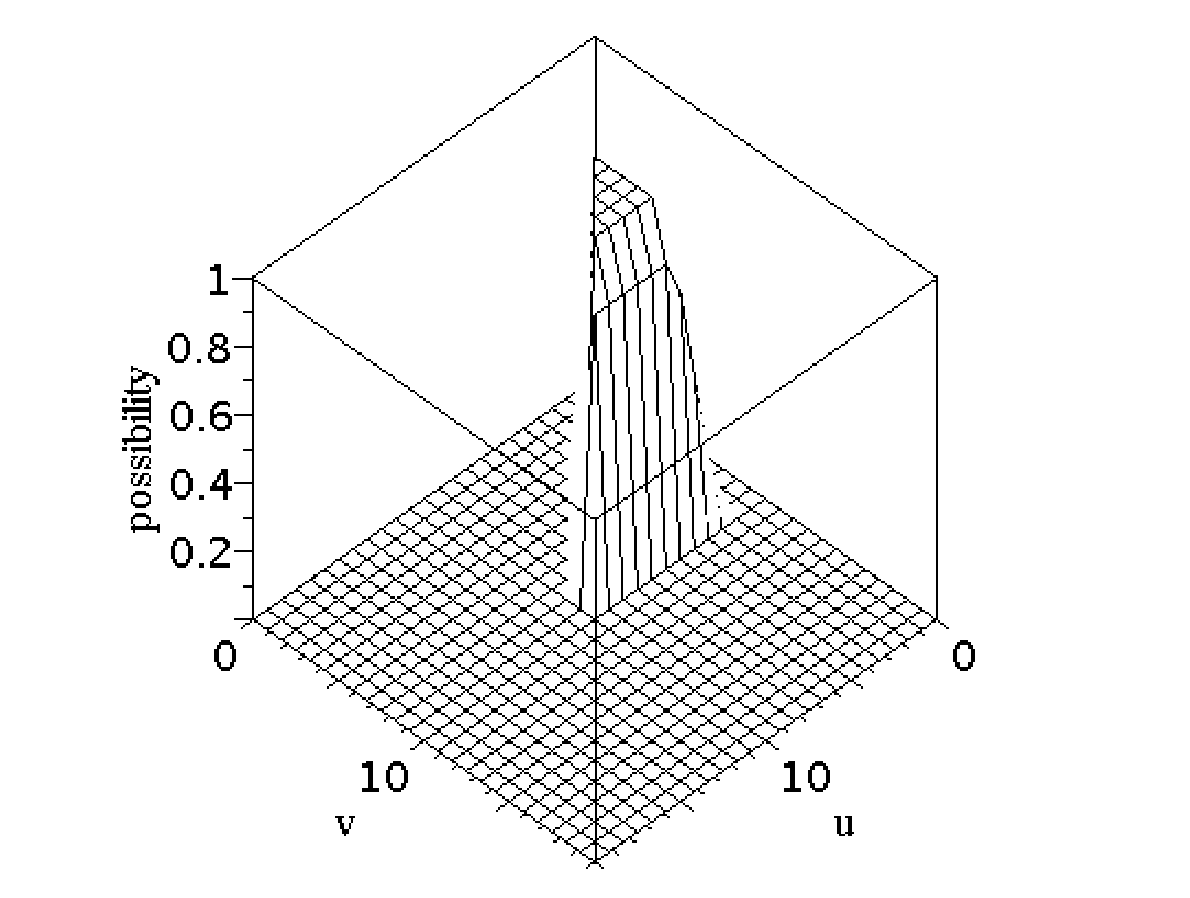
\includegraphics[scale=0.4]{graphs/3D_possibility.eps}
%\caption{Possibility of evaluation for the interval $[a,b]$.}
%\label{fig:3d-possibility}
%\end{figure}
%The necessity plot is obtained in a similar way and is shown in Figure~\ref{fig:3d-necessity}. Notice that the necessity measure is not normalized because the supports of $X$ and $Y$ overlap.
%\begin{figure}[h!]
%\centering
%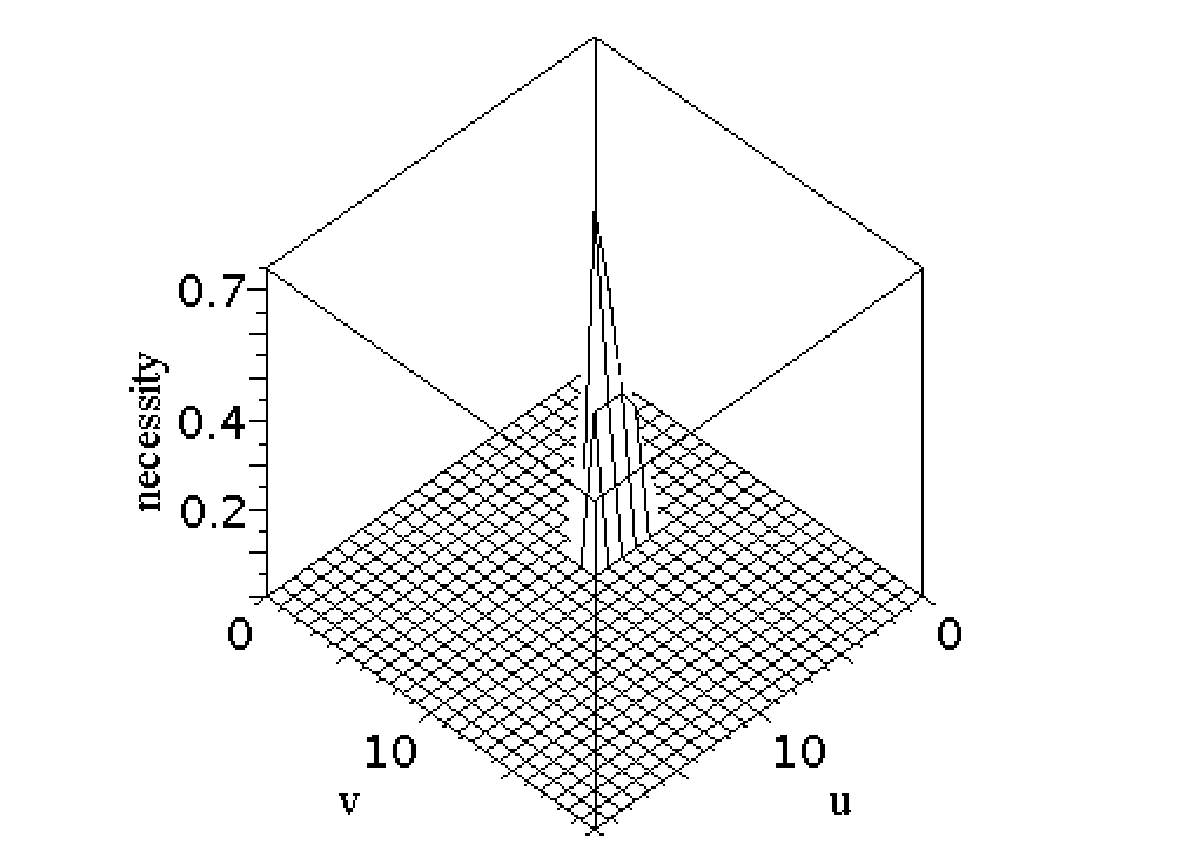
\includegraphics[scale=0.4]{graphs/3D_necessity.eps}
%\caption{Necessity of evaluation for the interval $[a,b]$.}
%\label{fig:3d-necessity}
%\end{figure}



\subsection{Temporal Databases}
%In this section, the proposed reasoning is applied to the specific context of intervals on the real line. This setting is of specific interest in the context of fuzzy temporal databases.
A \emph{temporal database} is a database that manages some aspects of time in its schema \cite{Dyreson1994}. The reality a temporal database tries to model, contains some temporal notions which have to be handled specifically in order to maintain a consistent modelling behavior. A \emph{chronon} is the shortest duration of time supported by the database. Time can be represented either as points~\cite{Dubois89} or intervals ~\cite{Garrido2009},\cite{655777} that may be subject to imperfection.
%There are proposals for the fuzzyfication of the time point and the fuzzyfication of the time interval.


%Time granularity is also associated with the representation of the time. A granularity is the result of partitioning on the set of chronons. The conversion among granularities is a common issue within temporal databases \cite{Lin97efficientconversion}. Granularity is the basis of some systems \cite{Cru97},\cite{624013}.

The temporal notions in temporal databases can be classified into 4 types based on their interpretation and modelling purpose. User-defined time has no interpretation, but the other types do:

\begin{itemize}
	\item
	\emph{Transaction time}~\cite{Jensen91}: The time when the fact is stored in the database.
	\item
	\emph{Valid time}~\cite{Snodgrass84}: The time when the fact is true in the modelled reality.
	\item
	\emph{Decision time}~\cite{Nascimento95}: The time when an event was decided to happen. 
\end{itemize}
	
Database models can also be classified into \emph{bi-temporal} (both valid and transaction-time) or \emph{tri-temporal}  (bi-temporal and decision time) models.


%To deal with time points  or intervals  that are subject to imperfection and can thus not be precisely known, fuzzy temporal models \cite{schockaert08} exist. %Some fuzzy temporal models assume that the time stored in the database is an interval. The temporal interval is represented by two ill-known time points: $X$  an ill-known starting point and $Y$ an ill-known ending point. The interval $\left[X,Y\right]$ is not a fuzzy interval but an ill-known interval: it is a crisp interval but it is partially unknown which values are in this interval.
